% Rapport de projet d'année - Pierre Gérard

\documentclass{article}

\usepackage[francais]{babel}
\usepackage[utf8x]{inputenc}
\usepackage[T1]{fontenc}
\usepackage{graphicx} % image
\usepackage{fancyhdr} % header
\usepackage{lastpage}
\usepackage{verbatim} %code
\usepackage{float} %float force [H](here)


% Marge et espace ---------------------------

\topmargin=0.1cm
\evensidemargin=0cm
\oddsidemargin=0cm
\textwidth=16.5cm
\textheight=21.5cm
\headsep=0.6cm

% ----- code ligne breaking alignement ------
% My question (Pierre)  : (http://tex.stackexchange.com/questions/86683/verb-end-of-the-line-alignement)
% Use : \texttt{\camelhyph{codePtythonIci}}

\makeatletter
\def\camelhyph#1{\c@melhyph#1\relax}
\def\c@melhyph#1{%
  \ifx#1\relax\else
    \ifx#1\-#1\else
      \ifnum`#1<91 \-\fi
      #1%
      \expandafter\expandafter\expandafter\c@melhyph\expandafter
    \fi
  \fi}
\makeatother

% definition  ----------------------

\newcommand{\rpTitre}{Rapport de projet}
\newcommand{\rpDate}{17 décembre 2012}
\newcommand{\rpCours}{INFO-F-106}
\newcommand{\rpProf}{V. BERTEN, O. MARKOWITCH, T. MASSART}
\newcommand{\rpAuteur}{Pierre Gérard}
\newcommand{\rpMatriculeULB}{000379259}


% header / footer -------------------

\pagestyle{fancy}
\lhead{\rpAuteur}
\chead{} 
\rhead{\rpCours\ : \rpTitre}
\lfoot{} 
\cfoot{- \thepage /\pageref{LastPage} -}
\rfoot{}



%Page de garde --------------

\title{
\vspace{5cm}
\textbf{\rpCours:\ \rpTitre}\\
\vspace{0.25cm}\small{ \rpDate}\\
\vspace{0.25cm}\large{\textit{Titulaires : \rpProf}}
\vspace{5cm}
}

\author{
\textbf{\rpAuteur} \\ 
\small{\rpMatriculeULB}
}
\date{} 


%rapport expliquant l'analyse, les dificultés rencontrées et les solutions proposées

\begin{document}

% garde
\maketitle
\newpage
% table
\tableofcontents
\newpage

% contenue
\chapter{}
\section{Introduction}
Afin d'appliquer et de développer les notions vues au cours de la première année de bachelier en sciences informatiques, il est demandé d'implémenter en langage Python3 une version légèrement simplifiée de la variante française du jeu de dames. 

\section{Présentation du problème}
La version simplifiée de la variante française du jeu de dames est pratiquement la même que la version française du jeu de dames à quelques exceptions. Les exceptions sont :
\begin{itemize}
    \item les prises ne sont pas toujours obligatoires, 
    \item il ne faut pas faire la plus grande prise possible,
    \item une dame doit s'arrêter après une pièce capturée si il y a eu capture.
\end{itemize}
L'objectif est d'implémenter cette version simplifiée du jeu de dames en Python3. Le programme est exclusivement en lignes de commandes et devra interagir avec deux utilisateurs qui rentreront chacun à leur tour le coup souhaité. ll permet aussi à l'utilisateur de sauvegarder ou restaurer une partie.

\section{Structure avec les règles}
Les fonctions implémentant la structure de base du damier et vérifiant la validité d'un coup par rapport aux règles se situent dans le fichier \texttt{\camelhyph{draughtsFunctions.py}}. Leurs noms et leurs fonctionnalités sont imposés. Les fonctions réalisent les actions suivantes :
\subsection{Initialisation du damier}
Le damier est composé de 10 cases sur 10 et chaque joueur possède 20 pions situés sur les cases blanches jouables. Le damier sera initialisé par la fonction \texttt{\camelhyph{initBoard}} qui s'occupe de placer les pions au bon endroit. En pratique, le damier est représenté par une liste contenant 10 sous-listes qui correspondent aux lignes. Ces sous-listes contiennent chacune 10 entiers qui correspondent aux pions. Une valeur de 0 équivaut à une case vide, une valeur négative à une pièce noire et une valeur positive à une pièce blanche. Le damier est donc une matrice.
\subsection{Affichage du damier}
Pour faciliter la lecture du damier, il est demandé d'écrire une fonction \texttt{\camelhyph{printBoard}} qui va imprimer un tableau de la façon suivante.

\begin{figure}[H]
\begin{center}
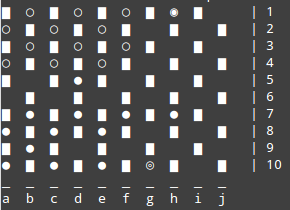
\includegraphics{printBoard.PNG}
\end{center}
\caption{Exemple d'affichage du damier lors du tour du joueur blanc}
\label{Exemple d'affichage du damier}
\end{figure}

La fonction va imprimer les pions du joueur en train de jouer en-dessous. Les différents pions sont représentés par un caractère unicode unique et il est considéré que le joueur joue dans un environnement console sur fond noir ce qui permet de différencier les pions blancs \og remplis\fg   des pions noirs \og non-remplis\fg .

\subsection{Vérification d'un coup}
L'implémentation de la vérification de la validité d'un coup et du respect des règles est la plus difficile à réaliser. Il faut gérer 12 erreurs différentes. La fonction \verb|checkMove| va vérifier que :
\begin{itemize}
	\item Le format de direction entré par le joueur est correct et est bien une des 4 possibilités.
	\item Il y a une pièce sur le damier à l'endroit qui correspond aux coordonnées entrées par le joueur.
	\item La pièce que le joueur essaie de déplacer lui appartient.
	\item Les nouvelles coordonnées après le déplacement souhaité par le joueur se situent bien sur le damier.
	\item Sur la case correspondant aux coordonnées que donnerait le déplacement, il n'y a pas de pièce appartenant au joueur, ce qui rendrait le déplacement impossible.
	\item Si sur la case correspondant aux coordonnées entrées par le joueur, il y a un pion, alors la longueur du déplacement doit être de une case. On peut aussi noter que cette erreur peut ne jamais se produire si on ne demande pas la longueur du déplacement au joueur quand il essaie de déplacer un pion.
	\item Si le déplacement entraine une capture, il faut que la case située après la pièce que le joueur essaie de capturer ne se trouve pas en dehors du damier.
	\item Le joueur n'essaie pas de sauter plusieurs pièces en un déplacement. Pour cela, il faut vérifier que après la première capture possible il y a une case libre.
	\item Si le joueur essaie de déplacer un pion en arrière, il doit y avoir capture.
	\item Si le joueur poursuit une rafle, le mouvement qu'il veut effectuer doit capturer une pièce. La même erreur est renvoyée si le joueur veut continuer à jouer alors qu'il n'a pas capturé lors de son premier déplacement. Cependant ce dernier cas ne se produit jamais si la fonction principale empêche le joueur de rejouer si il ne capture pas de pièce.
	\item Si le joueur déplace une dame, elle ne passe pas au-dessus de plusieurs pions. Pour cela, la fonction fait appel à une autre fonction \verb|countFree| qui renvoie le nombre de pièces jusqu'au premier obstacle (bord ou pion). Ensuite, elle vérifie que ce nombre n'est pas inférieur à la longueur du déplacement.%
\end{itemize}
Sinon la fonction renvoie qu'il n'y a pas d'erreurs et le joueur peut effectuer son mouvement. Elle renvoie en réalité un code d'erreur numérique différent pour chaque erreur. Ce code numérique sera traduit au joueur par la fonction \texttt{\camelhyph{sterr}}
\subsection{Déplacement d'un pion et capture}
Lorsque qu'un déplacement est vérifié, le programme peut modifier la matrice représentant le damier pour que le déplacement soit effectué. C'est la fonction \texttt{\camelhyph{movePiece}} qui va s'en occuper. Elle va ensuite renvoyer les coordonnées de la destination du pion et les coordonnées de la pièce capturée si il y en a une et \texttt{\camelhyph{None}} sinon. Ensuite si il y a eu capture, la fonction principale va appeler la fonction \texttt{\camelhyph{capture}} qui va enlever la pièce du damier.
\subsection{Détection de la fin de la partie et du gagnant}
Une partie est terminée lorsque un joueur ne sait plus bouger ou n'a plus de pièces. C'est alors son adversaire qui remporte la partie. La fonction \texttt{\camelhyph{checkEndOfGame}} permet de détecter ces différents cas. Pour cela, elle appelle la fonction \texttt{\camelhyph{checkEndOfGameForPlayer}} qui détecte si le joueur passé en paramètre possède encore une pièce et si il sait faire un mouvement. Elle effectue cette dernière tâche en appelant la fonction qui vérifie un coup en testant les 4 directions possibles jusqu'à ce qu'elle trouve une possibilité qui fonctionne si il y en a une. Ensuite, elle renvoie ce résultat. La fonction initiale de vérification va ensuite faire de même pour l'autre joueur et analyser les différents résultats. Elle pourra ensuite renvoyer le résultat; le joueur gagnant, un match nul ou bien une partie pas encore terminée.

Cependant cette fonction ne détecte pas les parties sans fin. C'est pourquoi la partie du programme qui interagit avec les joueurs leur permet de proposer à l'adversaire un match nul.
\subsection{Sauvegarde et restauration d'une partie}
Pour rajouter des fonctionnalités au jeu, il est aussi demandé d'implémenter un système de sauvegarde et de restauration de la partie en cours. Ce sont respectivement les fonctions \texttt{\camelhyph{save}} et \texttt{\camelhyph{load}} qui vont s'en occuper. Ces deux fonctions vont écrire et lire sur un fichier dont le format \texttt{\camelhyph{.dat}} est imposé, à savoir le joueur qui doit jouer le prochain coup, la taille du damier,  et le damier lui-même.
\section{Interaction avec l'utilisateur et fonction principale}
La fonction principale et les interactions avec les joueurs sont contrôlées par les fonctions situées dans le fichier \verb|draughts.py|. Il est important de considérer que l'utilisateur peut se tromper en entrant des données. Ces erreurs pouvant nuire à la bonne éxecution du programme, il est important de les gérer.

La fonction principale joue le rôle de chef d'orchestre du programme. En effet, c'est elle qui va permettre à l'utilisateur de jouer en interagissant avec lui et la structure de base et les règles. Elle est structurée et peut se résumer de la manière suivante :

\begin{verbatim}
Initialiser le damier
Joueur = joueur blanc
Tant que le jeu n'est pas fini:
    Imprimer le damier et le joueur qui a le trait
    choix = ce que le joueur veut faire
    Si choix == déplacer une pièce :
        Tant que le déplacement n'est pas valide :
            Demander le premier déplacement souhaité.
        Effectuer le déplacement
        Si pas de capture:
            Indiquer au joueur pas de capture
        Sinon:
            Demander au joueur si il veut poursuivre sa rafle
            Tant que le joueur souhaite poursuivre sa rafle:
                Demander le déplacement et vérifier sa validité
                Effectuer le déplacement si il est valide
                Redemander joueur si il veut poursuivre sa rafle
        Passer à l'autre joueur
        Vérifier la fin du jeu
    Sinon si choix == proposer un match nul à l'adversaire:
        Demander à l'autre joueur si il accepte
    Sinon si choix == sauvegarder :
        Sauvegarder une partie
    Sinon si choix == restaurer :
        Restaurer une partie
\end{verbatim}

\subsection{Initialisation du damier}
La fonction principale initialise le damier en appelant la fonction principale et lève une exception si la configuration demande de créer une taille de damier inférieure à 4.
\subsection{Impressions}
Pour rendre l'affichage du jeu plus simple, la fonction principale appelle en plus de la fonction \texttt{\camelhyph{printBoard}} deux autres fonctions qui permettent d'imprimer de manière plus esthétique le joueur qui a le trait et le pion capturé. Il s'agit respectivement de \texttt{\camelhyph{printCurrentPlayer}} et \texttt{\camelhyph{printCapture}}.

\subsection{Choix de l'action}
Le programme laisse à l'utilisateur le choix de l'action à effectuer. Il lui pose la question et il répond par 1,2,3 ou 4 en fonction de l'action qu'il souhaite effectuer. Les actions possibles sont respectivement: déplacer une pièce, proposer un match nul à l'adversaire, sauvegarder la partie ou bien restaurer la partie. C'est la fonction \texttt{\camelhyph{inputActionChoice}} qui va vérifier si le choix est correct.
\subsection{Premier déplacement}
Si un joueur souhaite déplacer une pièce, le programme va lui demander d'entrer les coordonnées du déplacement via la fonction \texttt{\camelhyph{inputCoordinates}}. Cette dernière demande les coordonnées à l'utilisateur de manière simplifiée (exemple (j,4)) et la direction du déplacement. Elle est aussi optimisée pour ne demander la longueur du déplacement que si c'est une dame qui est située à cet endroit-là. Elle va ensuite vérifier ce déplacement et l'effectuer. Si le déplacement n'est pas correct, elle va lui en redemander un nouveau jusqu'à ce que qu'il en rentre un correct.
\subsection{Rafle}
Si le joueur effectue une capture lors du premier déplacement de son coup, alors le programme va lui demander si il souhaite poursuivre une rafle. Si il répond \og oui\fg  le programme va lui demander la direction du mouvement et la longueur si c'est une dame via la fonction \texttt{\camelhyph{inputCooAfterCapture}}. Le programme va continuer de lui poser la question tant que le joueur effectue une capture.
\subsection{Sauvegarde d'une partie}
Lorsque le joueur souhaite sauvegarder une partie, le programme va lui demander d'entrer le nom qu'il souhaite donner au fichier de sauvegarder et va ensuite ajouter l'extension \texttt{\camelhyph{.dat}} à ce dernier et le sauver. Il va ensuite lui demander si il veut continuer à jouer ou si il veut s'arrêter là et reprendre une autre fois. Il se peut qu'il y ait un problème lors de la sauvegarde et qu'une exception de type \texttt{\camelhyph{IOError}} soit levée. Dans ce cas, le programme va le signaler à l'utilisateur et lui redemander l'action qu'il souhaite faire.
\subsection{Restauration d'une partie}
Lorsque le joueur souhaite charger une partie, le programme va lui demander le nom du fichier de sauvegarde et va ensuite ajouter l'extension \texttt{\camelhyph{.dat}} à ce dernier et essayer de charger le fichier. Il se peut qu'il y ait un problème lors du chargement (fichier inexistant, pas de droit d'accès, ...) et qu'une exception de type \texttt{\camelhyph{IOError}} soit levée. Il se peut aussi que la fonction lève une autre exception si il y a eu des altérations de données dans le fichier de sauvegarde. Dans ce cas, le programme va récupérer cette exception et dire à l'utilisateur que le fichier qu'il essaie de charger est corrompu. Le chargement du fichier permet de récupérer le damier et le joueur qui a le trait.

\section{Exemples de résultats}

\subsection{Mouvement en milieu de partie}
Lorsque par exemple le joueur noir essaie de déplacer un pion située en (i,4) vers la droite, il le fait de la manière suivante :
\begin{verbatim} 
C'est au tour du joueur avec les pièces noires
Souhaitez vous :
1) Déplacer une pièce 
2) Proposer une partie nulle à l'adversaire
3) Sauvegarder la partie 
4) Restaurer la partie
  Entrez votre choix : 1
Veuillez répondre par 1,2,3 ou 4 : 
Entrez la coordonnées en x [a-j] : i
Entrez la coordonnées en y [1-10] : 4
Entrez la direction souhaité : r
Vous déplacer une pièce sans effectuer de capture
C'est au tour du joueur avec les pièces blanches
\end{verbatim}
On remarque que la pièce est désormais en (i,5)

\subsection{Fin de partie par une rafle}
Pour le damier suivant :
\begin{figure}[H]
\begin{center}
\includegraphics{exemple.PNG}
\end{center}
\caption{Exemple de damier}
\label{Exemple de damier}
\end{figure}
Le joueur avec les pièces noires remarque qu'il peut gagner si il effectue une rafle de la manière suivante :
\begin{verbatim}
C'est au tour du joueur avec les pièces noires 
Souhaitez vous :
1) Déplacer une pièce 
2) Proposer une partie nulle à l'adversaire
3) Sauvegarder la partie 
4) Restaurer la partie
  Entrez votre choix : 1
Veuillez répondre par 1,2,3 ou 4 : 
Entrez la coordonnées en x [a-j] : i
Entrez la coordonnées en y [1-10] : 4
Entrez la direction souhaité : l
Entrez la longueur du déplacement : 2
Votre déplacement n'est pas correct : 
Vous ne pouvez pas déplacer une pièce à l’extérieur du damier
Entrez la coordonnées en x [a-j] : i
Entrez la coordonnées en y [1-10] : 4
Entrez la direction souhaité : r
Entrez la longueur du déplacement : 2
Vous avez capturé la pièce adverse situé en (g,6)
[impression nouveau damier]
Souhaitez-vous poursuivre une rafle ? o/n : 
o
Entrez la direction souhaité : r
Entrez la longueur du déplacement : 1
Vous avez capturé la pièce adverse situé en (e,8)
[impression nouveau damier]  
Le jeu se termine par la victoire du joueur avec les pions noirs
\end{verbatim}

\section{Conclusion}

Le programme implémente bien une version simplifié du jeu de dames fonctionnelle. Cependant, cette version est entièrement en lignes de commandes et ne rend donc pas le jeu très convivial.

\end{document}